\documentclass[11pt]{article}
\usepackage[margin=1in]{geometry}
\usepackage{amsmath,amssymb,amsthm,booktabs,graphicx,hyperref,array,microtype,enumitem}
\usepackage{xcolor}
\hypersetup{colorlinks=true,linkcolor=blue!50!black,urlcolor=blue!50!black,citecolor=blue!50!black}
\newcommand{\FibTotal}{99}
\newcommand{\FibConst}{9}
\newcommand{\FibAff}{14}
\newcommand{\FibQuad}{15}
\newcommand{\FibClosed}{38}
\newcommand{\FibRec}{61}
\newcommand{\FibClosedPct}{38.4}
\newcommand{\SqDTotal}{105}
\newcommand{\SqDConst}{23}
\newcommand{\SqDAff}{27}
\newcommand{\SqDQuad}{37}
\newcommand{\SqDClosed}{87}
\newcommand{\SqDRec}{18}
\newcommand{\SqDClosedPct}{82.9}
\newcommand{\SqWTotal}{64}
\newcommand{\SqWConst}{16}
\newcommand{\SqWAff}{22}
\newcommand{\SqWQuad}{23}
\newcommand{\SqWClosed}{61}
\newcommand{\SqWRec}{3}
\newcommand{\SqWClosedPct}{95.3}
\newcommand{\FibIterB}{2\,273\,316}
\newcommand{\FibIterK}{1\,398\,227}
\newcommand{\FibIterRed}{38.5}
\newcommand{\FibRecB}{7\,194}
\newcommand{\FibRecK}{4\,429}
\newcommand{\FibRecRed}{38.4}
\newcommand{\FibOpsB}{33\,994\,872}
\newcommand{\FibOpsK}{23\,489\,360}
\newcommand{\FibOpsRed}{30.9}
\newcommand{\FibShort}{2\,765}
\newcommand{\SqDIterB}{270\,247}
\newcommand{\SqDIterK}{59\,724}
\newcommand{\SqDIterRed}{77.9}
\newcommand{\SqDRecB}{18\,335}
\newcommand{\SqDRecK}{4\,073}
\newcommand{\SqDRecRed}{77.8}
\newcommand{\SqDOpsB}{698\,762}
\newcommand{\SqDOpsK}{251\,240}
\newcommand{\SqDOpsRed}{64.0}
\newcommand{\SqDShort}{14\,262}
\newcommand{\SqWIterB}{474\,635}
\newcommand{\SqWIterK}{36\,990}
\newcommand{\SqWIterRed}{92.2}
\newcommand{\SqWRecB}{26\,711}
\newcommand{\SqWRecK}{2\,040}
\newcommand{\SqWRecRed}{92.4}
\newcommand{\SqWOpsB}{847\,876}
\newcommand{\SqWOpsK}{168\,800}
\newcommand{\SqWOpsRed}{80.1}
\newcommand{\SqWShort}{24\,671}
\newcommand{\FibInputs}{900}
\newcommand{\FibRouteInputs}{872}
\newcommand{\FibSmallInputs}{28}
\newcommand{\FibRejects}{4\,111}
\newcommand{\FibMaxIterB}{8\,280}
\newcommand{\FibMaxIterK}{4\,912}
\newcommand{\SqDInputs}{5\,435}
\newcommand{\SqDRejects}{2\,952}
\newcommand{\SqDMaxMoves}{5}
\newcommand{\SqWInputs}{5\,435}
\newcommand{\SqWRejects}{2\,952}
\newcommand{\SqWMaxMoves}{8}
\newcommand{\FibMaxMoves}{12}
\newcommand{\CtrlFib}{201}
\newcommand{\CtrlSqD}{85}
\newcommand{\CtrlSqW}{45}
\newcommand{\ConstAll}{48}
\newcommand{\AffAll}{63}
\newcommand{\QuadAll}{75}
\newcommand{\ClosedAll}{186}
\newcommand{\RecAll}{82}
\newcommand{\StepsAll}{268}
\newcommand{\FibMeanRecB}{8.25}
\newcommand{\FibMeanRecK}{5.08}
\newcommand{\FibRegress}{0}
\newcommand{\FibRouteN}{872}
\newcommand{\SqDMeanRecB}{3.37}
\newcommand{\SqDMeanRecK}{0.75}
\newcommand{\SqDRegress}{0}
\newcommand{\SqDRouteN}{5\,435}
\newcommand{\SqWMeanRecB}{4.91}
\newcommand{\SqWMeanRecK}{0.38}
\newcommand{\SqWRegress}{0}
\newcommand{\SqWRouteN}{5\,435}
\newcommand{\NonClosed}{82}
\newcommand{\FieldFib}{51}
\newcommand{\FieldSq}{21}
\newcommand{\FieldNotPowTwo}{42}
\newcommand{\FieldPowTwo}{30}
\newcommand{\TenDegMin}{8}
\newcommand{\TenDegMax}{16}
\newcommand{\VerifierSha}{ed11ffccf7d69590}

\newtheorem{theorem}{Theorem}
\newtheorem{proposition}[theorem]{Proposition}
\newtheorem{lemma}[theorem]{Lemma}
\theoremstyle{definition}
\newtheorem{definition}[theorem]{Definition}
\theoremstyle{remark}
\newtheorem{remark}[theorem]{Remark}
\newcommand{\Q}{\mathbb{Q}}
\DeclareMathOperator{\isqrt}{isqrt}
\title{\textbf{UNNS-U2-KI}\\[2pt]\large Exact Knowledge Identities and Selector Reduction}
\author{UNNS Research Collective}
\date{Version v001 \quad (addendum to UNNS-U2-FP-R3 v001; that package, UNNS-U2-FP-SYM, UNNS-U2-FP, U2-SQ, U2-001 and U1-BND are unchanged)}
\begin{document}
\maketitle
\begin{abstract}
\noindent
UNNS-U2-FP-R3 classified the route labels of three finite-control selectors (Fibonacci successor, squares direct, squares wrapper) by interpolation at sample points. This addendum replaces those sample fits by exact statements. \textbf{KI-1.} For all \StepsAll{} audited route steps the classification is re-derived symbolically and agrees with the sample fits in every case; \ClosedAll{} steps have a certified state-only formula ($\ConstAll$ constants, $\AffAll$ affine in the state, $\QuadAll$ with a single integer square root of an affine function of the state), including a constant-sign certificate for the root branch. \textbf{KI-2.} For each of the remaining \NonClosed{} steps we compute the exact degree $d$ of the label over the field generated by the state. All have $d\ge 3$, so none is given by a rational function of the state or by one square root. The ten labels left unexplained in R3 have $d\in[\TenDegMin,\TenDegMax]$ and, by a Galois-group certificate, lie in no tower of square roots over the state either. \textbf{KI-3.} Controllers that execute only the certified shortcuts, built beside the unchanged R3 baseline, reproduce every baseline move sequence and every legal transition on identical inputs, and cut parameter recoveries by \FibRecRed\% (Fibonacci), \SqDRecRed\% (squares direct) and \SqWRecRed\% (squares wrapper). No input became more expensive. The Fibonacci selector still needs bisection at \FibRec{} of its \FibTotal{} steps, so the exact result sharpens the ledger rather than removing the controller's contribution. Nothing here concerns prime generation, target-independent selection, or classes of formula beyond those defined in Section~\ref{sec:classes}.
\end{abstract}

\section{Scope and evidence levels}
All earlier releases stay frozen. The R3 controllers are imported unchanged from a hashed copy (\texttt{baseline\_R3\_frozen/}); the optimized controllers are separate code. Statements are kept in three groups.
\begin{itemize}\setlength\itemsep{1pt}
\item \emph{Certified exactly}: polynomial identities in the free module $\Q[b]\oplus\Q[b]\,a$ or in $\Q[t]$ (SymPy, no proof assistant); constant-sign tests by Sturm root counting; exact rank statements; identities in $\Q(m)$ checked at more points than their degree bound.
\item \emph{Certified up to a cited standard theorem}: the radical-tower exclusion (Section~\ref{sec:tower}), whose machine-computed certificate is a factorization pattern modulo a prime.
\item \emph{Tested}: exhaustive or deterministic runs of the implemented selectors (Section~\ref{sec:ki3}).
\end{itemize}
``Not found in a vocabulary'' is never read as necessity. Necessity is claimed only where Section~\ref{sec:ki2} proves nonexistence in a formally defined class.

\section{Setting}\label{sec:setting}
The graph $G$ has edges $\{kN,\,k(N+1)^2\}$; the move $+N$ sends $x\mapsto x(N+1)^2/N$ (needs $N\mid x$), the move $-N$ sends $x\mapsto xN/(N+1)^2$ (needs $(N+1)^2\mid x$). A route class of a selector is a finite sequence of signed labels $N_0,\dots,N_{\ell-1}$ with states $S_0,\dots,S_{\ell-1}$ (the integer before the move), each a function of a class parameter.

\paragraph{Fibonacci ring.} With $(a,b)=(F_{h-1},F_h)$ and $\varepsilon=(-1)^h$ we have $a^2+ab-b^2=\varepsilon$. Route states and labels of the twelve FP-SYM classes are elements of $R_\varepsilon=\Q[b][a]/(a^2+ab-b^2-\varepsilon)$, a free $\Q[b]$-module with basis $\{1,a\}$. An element is zero iff its two coefficient polynomials vanish. Writing $X=2a+b$, $Y=b$, the relation reads $X^2-5Y^2=4\varepsilon$, a conic with a rational point, so its function field $K_\varepsilon$ is a rational function field $\Q(m)$ (for $\varepsilon=1$: $Y=4m/(5-m^2)$, $X=(10+2m^2)/(5-m^2)$; for $\varepsilon=-1$: $Y=(m^2-2m+5)/(m^2-5)$, $X=(-m^2+10m-5)/(m^2-5)$). For the two square families the ring is $\Q[t]$ and $K=\Q(t)$ ($m:=t$). States are $S_0=n^2$ with $n=24t+r$ (direct) and $S_0=(m_0+1)^2$ with the U2-001 identities for $m_0=Mt+r$ (wrapper).

\paragraph{Authorized primitives (R3$'$).} Exact integer $+,-,\times$, exact division by constants, comparison, $\isqrt$, and residues modulo a fixed modulus. R3$'$ itself is not changed by this addendum, and no selector below uses anything else.

\section{Expression classes and degree}\label{sec:classes}
Fix a step with state $S$ and label $N$, both elements of $K=\Q(m)$. Because $K$ has transcendence degree one, $S$ and $N$ are algebraically dependent; let $F(n,s)\in\Q[n,s]$ be an irreducible polynomial with $F(N,S)=0$ and put
\[ d(N\mid S)\;=\;[\Q(S,N):\Q(S)]\;=\;\deg_n F. \]
A \emph{direct-state formula} for $N$ is an expression in $S$ built from the authorized primitives with rational constants. We use three nested classes.
\begin{itemize}\setlength\itemsep{1pt}
\item $\mathcal C_1$: $N=R(S)$ with $R\in\Q(X)$ (division only).
\item $\mathcal C_2$: $N$ is a root of a quadratic polynomial over $\Q(S)$, i.e.\ one $\isqrt$ of a rational function of $S$.
\item $\mathcal C_3$: $N$ lies in a finite tower of quadratic extensions of $\Q(S)$, i.e.\ iterated $\isqrt$.
\end{itemize}
Then $\mathcal C_1$ means $d=1$, $\mathcal C_2$ means $d\le 2$, and $\mathcal C_3$ forces $d$ to be a power of two and the Galois group of $F(\cdot,S)$ over $\Q(S)$ to be a $2$-group. A formula that is exact on infinitely many class members is an algebraic identity, up to finitely many branch choices; so the classes describe what such formulas can be, not only what we searched.

Formulas outside these classes (searches, bisection, residue or gcd tests, use of other history) are not covered, and the nonexistence statements below say nothing about them.

\section{KI-1: exact identities}\label{sec:ki1}
\begin{lemma}[sign of $u+v\alpha$]\label{lem:sign}
Let $\alpha=(\sqrt D-b)/2$ with $D=5b^2+4\varepsilon>0$, and $E=e_0(b)+e_1(b)\alpha$ with $e_0,e_1\in\Q[b]$. Put $P=2e_0-be_1$, $Q=e_1$, so $E=(P+Q\sqrt D)/2$. If $P$, $Q$ and, when their signs differ, $P^2-Q^2D$ each have no real root on $[40,\infty)$, then $E$ has a constant nonzero sign on $[40,\infty)$, namely the common sign of $P,Q$, or, for opposite signs, the sign of whichever of $P,Q$ dominates according to the sign of $P^2-Q^2D$.
\end{lemma}
Each polynomial test is exact: a polynomial $p$ has no real root on $[b_0,\infty)$ iff $p(b_0)\neq 0$ and its Sturm count on $[b_0,\infty)$ is zero. The same test with $\Q[t]$ and $t\ge t_0$ is used for the square families, where $t_0$ is the start of validity of the class.

\begin{theorem}[exact shortcuts]\label{thm:ki1}
For each route step let $(S,N)$ be the symbolic state and label. Exactly one of the following holds in the audited vocabulary, and it is verified as an identity in $R_\varepsilon$ (Fibonacci) or $\Q[t]$ (squares), for all real $b\ge 40$ resp.\ $t\ge t_0$:
\begin{enumerate}[label=(\alph*),itemsep=1pt]
\item $N=c$ (constant);
\item $N=c_0+c_1S$ with $c_0,c_1\in\Q$;
\item $k_{20}N^2+k_{10}N+k_{00}+k_{01}S=0$ with integers $k_{ij}$, $k_{20}>0$; moreover $W:=2k_{20}N+k_{10}$ satisfies $W^2=\Delta(S):=k_{10}^2-4k_{20}(k_{00}+k_{01}S)$ and $W>0$ on the whole domain, so
\[ N\;=\;\frac{\sqrt{\Delta(S)}-k_{10}}{2k_{20}}\qquad\text{and at integer points }\sqrt{\Delta}=\isqrt\Delta. \]
\end{enumerate}
\end{theorem}
\emph{Proof.} (a)--(c) are linear problems for the unknown coefficients: the coefficient polynomials of $N-c_1S-c_0$ (resp.\ of the relation) in the basis $\{1,a\}$ must vanish. SymPy solves these exactly; each solution is then substituted and every coefficient is checked to be the zero polynomial. For (c), $4k_{20}\cdot(\text{relation})=W^2-\Delta(S)$ gives $W^2=\Delta$ once the relation holds, and the identity is also checked directly. Positivity of $k_{20}=A_2$ and of $W$ on the domain is Lemma~\ref{lem:sign}. \hfill$\square$

\begin{table}[h]\centering\small
\caption{Exact classification of all audited steps. ``Recovery'' = no formula of type (a)--(c); see KI-2. Counts agree with the R3 sample fits in every one of \StepsAll{} cases.}
\begin{tabular}{@{}lrrrrrr@{}}\toprule
selector & steps & constant & affine & one $\isqrt$ & closed form & recovery\\\midrule
Fibonacci & \FibTotal & \FibConst & \FibAff & \FibQuad & \FibClosed{} (\FibClosedPct\%) & \FibRec\\
Squares direct & \SqDTotal & \SqDConst & \SqDAff & \SqDQuad & \SqDClosed{} (\SqDClosedPct\%) & \SqDRec\\
Squares wrapper & \SqWTotal & \SqWConst & \SqWAff & \SqWQuad & \SqWClosed{} (\SqWClosedPct\%) & \SqWRec\\\bottomrule
\end{tabular}
\end{table}

\noindent All $\QuadAll$ relations of type (c) have $k_{11}=k_{21}=0$, so $\Delta$ is affine in $S$ and a single $\isqrt$ of an affine function of the state suffices; the branch sign is $+$ in every case. Examples (Fibonacci, class $0$): step~$1$ is $N=S/4$; step~$6$ is $4N^2+8N+4=S$, i.e.\ $N=(\isqrt S-2)/2$. The percentages \FibClosedPct, \SqDClosedPct{} and \SqWClosedPct{} quoted in R3 are therefore now exact statements about these route families, not sample-fitted ones. The full coefficient table is \texttt{data/ki1\_identities.json}.

\begin{figure}[h]\centering
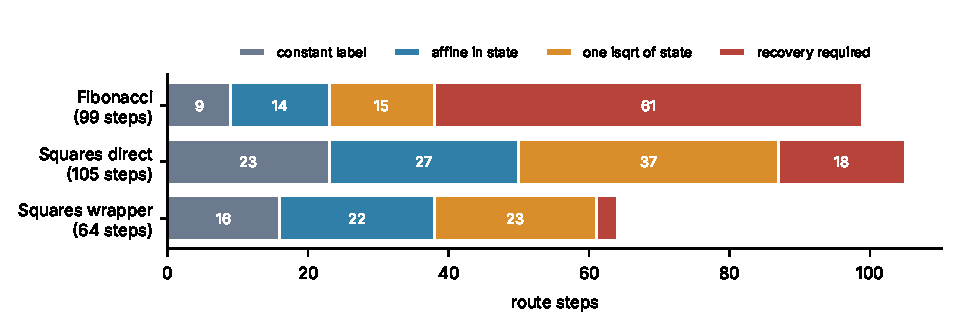
\includegraphics[width=0.92\textwidth]{../figures/fig1_categories.pdf}
\caption{Exact knowledge categories of the \StepsAll{} route steps (KI-1).}
\end{figure}

\section{KI-2: dependence versus necessity}\label{sec:ki2}
\subsection{Exact degrees}
For each of the \NonClosed{} steps without a formula we computed $d=d(N\mid S)$. Lower bound: a relation $\sum_{i\le d',j\le \deg_mN}k_{ij}N^iS^j=0$ with $d'<d$ would vanish at every sample point of the curve $m\mapsto(N,S)$; the evaluation matrices have trivial nullspace modulo $2^{61}-1$, hence over $\Q$. (The bound $j\le\deg_mN$ is the full range: $\deg_s F\le[\Q(m):\Q(N)]=\deg_mN$.) Upper bound: the relation of degree $d$ found over $\Q$ is an identity in $\Q(m)$, verified at more points than its numerator degree. All \NonClosed{} existence checks passed.

\begin{table}[h]\centering\small
\caption{Exact degree $d$ of the label over $\Q(S)$ for the steps without a formula; ``field'' and ``unexplained'' are the R3 audit classes.}
\begin{tabular}{@{}lrrrrrrrr@{}}\toprule family / audit class & $d{=}3$ & $4$ & $6$ & $8$ & $10$ & $12$ & $14$ & $16$ \\\midrule
Fibonacci, \emph{field} & 2 & 21 & 22 & 4 & 1 & -- & 1 & -- \\
Fibonacci, \emph{unexplained} & -- & -- & -- & 1 & 3 & 3 & 2 & 1 \\
Squares (direct + wrapper), \emph{field} & 16 & 5 & -- & -- & -- & -- & -- & -- \\
\bottomrule\end{tabular}

\end{table}

\begin{theorem}[no formula in $\mathcal C_1\cup\mathcal C_2$]\label{thm:c2}
All \NonClosed{} steps without a KI-1 formula have $d\ge 3$. Hence none lies in $\mathcal C_1$ or $\mathcal C_2$: no rational function of the state, and no expression with one square root, gives the label on these route classes.
\end{theorem}

\subsection{The ten unresolved Fibonacci labels}\label{sec:tower}
R3 left ten labels (classes $1$ and $9$) unexplained in its vocabulary. Their exact degrees are $d\in\{8,10,10,10,12,12,12,14,14,16\}$ (Table~\ref{tab:ten}).
\begin{proposition}[radical towers]\label{prop:tower}
None of the ten labels lies in $\mathcal C_3$.
\end{proposition}
\emph{Argument.} For each, $\deg_mN=2$ while the minimal relation has $\deg_sF=2$, so $\Q(S,N)=\Q(m)=K$ and $d=\deg_mS$; the Galois closure of the minimal polynomial of $N$ over $\Q(S)$ is the splitting field of $f(m;s)=\mathrm{num}\,S(m)-s\,\mathrm{den}\,S(m)$ over $\Q(s)$. If $N$ lay in a tower of quadratic extensions this group $G$ would be a $2$-group. For $d=10,12,14$ that already fails ($d$ is not a power of two). For $d=8,16$ and for uniformity in all ten, the table lists a prime $p$ and an integer $s_0$ for which $f(m;s_0)\bmod p$ is squarefree with factor degrees whose least common multiple is divisible by an odd prime. By Dedekind's factorization theorem for unramified specializations, $G$ then contains an element of order divisible by that prime, so $G$ is not a $2$-group. The factorizations are machine-computed; the passage from them to $G$ is a standard theorem, not machine-checked. \hfill$\square$

\begin{table}[h]\centering\small
\caption{The ten unresolved labels: degrees of label and state in the conic parameter $m$, exact degree $d$ over $\Q(S)$, and the specialization certificate.}\label{tab:ten}
\begin{tabular}{@{}rrrrrll@{}}\toprule class & step & $\deg_m N$ & $\deg_m S$ & $d$ & $(p,s_0)$ & factor degrees of $S(m)=s_0 \bmod p$ \\\midrule
1 & 2 & 2 & 12 & 12 & (10007,2) & {\footnotesize $1,1,2,2,3,3$}; order 6 \\
1 & 3 & 2 & 14 & 14 & (10007,2) & {\footnotesize $1,3,3,7$}; order 21 \\
1 & 4 & 2 & 16 & 16 & (10007,2) & {\footnotesize $1,6,9$}; order 18 \\
1 & 6 & 2 & 10 & 10 & (10007,2) & {\footnotesize $1,3,6$}; order 6 \\
1 & 7 & 2 & 8 & 8 & (10007,2) & {\footnotesize $1,7$}; order 7 \\
1 & 8 & 2 & 10 & 10 & (10007,3) & {\footnotesize $2,2,6$}; order 6 \\
9 & 2 & 2 & 12 & 12 & (10007,2) & {\footnotesize $1,1,2,2,3,3$}; order 6 \\
9 & 3 & 2 & 10 & 10 & (10007,2) & {\footnotesize $1,2,2,5$}; order 10 \\
9 & 4 & 2 & 12 & 12 & (10007,3) & {\footnotesize $1,1,2,2,6$}; order 6 \\
9 & 5 & 2 & 14 & 14 & (10007,2) & {\footnotesize $1,13$}; order 13 \\
\bottomrule\end{tabular}

\end{table}

\paragraph{Reading the asymmetry.} For all ten, the label has degree~$2$ in the conic parameter while the state has degree $8$--$16$, and $S$ is quadratic over $\Q(N)$: the forward direction (label $\to$ state) is as cheap as one square root, the inverse direction has degree $d\ge8$. In these route classes the controller therefore receives the \emph{state} from the graph move but must \emph{recover} the label through its algebraic knowledge of the parametrization.

\subsection{Three outcomes}
\begin{center}\small
\begin{tabular}{@{}p{0.30\textwidth}p{0.10\textwidth}p{0.50\textwidth}@{}}\toprule
outcome & steps & scope of the statement\\\midrule
proved direct-state formula & \ClosedAll & Theorem~\ref{thm:ki1}, all three selectors\\
proved nonexistence in $\mathcal C_1\cup\mathcal C_2\cup\mathcal C_3$ & 10 & the ten labels (Prop.~\ref{prop:tower})\\
proved nonexistence in $\mathcal C_1\cup\mathcal C_2$ only & 72 & remaining Fibonacci (\FieldFib) and square (\FieldSq) steps; for \FieldNotPowTwo{} of them $d$ is not a power of two, so $\mathcal C_3$ is excluded as well; for \FieldPowTwo{} ($d=4$ or $8$) the tower question was not analysed\\\bottomrule
\end{tabular}
\end{center}
\begin{figure}[h]\centering
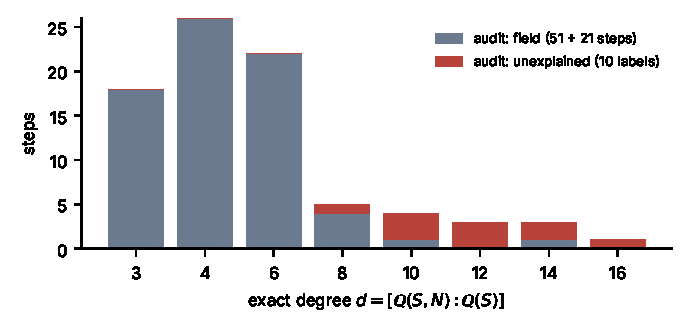
\includegraphics[width=0.62\textwidth]{../figures/fig3_degrees.pdf}
\caption{Exact degree of the label over the state for the \NonClosed{} steps without a formula.}
\end{figure}
\paragraph{Limits of these results.} Degrees are those of \emph{this} certified route family; another waypoint scheme between $F_k$ and $F_{k+1}$ could carry state-local labels where this one does not. The classes exclude, e.g., formulas using residues or search. No claim is made about primes.

\section{KI-3: selector reduction}\label{sec:ki3}
\paragraph{Construction.} The optimized controllers are separate code. Membership test, fixed-modulus dispatch, route tables, small-index table and graph edges are those of R3. At a step with a certified formula (a)--(c) the label is computed from the current integer; at the remaining steps the R3 recovery is called unchanged. At the first step of the squares selectors, and in the special-case tables, R3 never recovers a parameter, so those steps are left as they were. Each shortcut carries an arithmetic guard (perfect-square and divisibility checks) and raises an error if violated; no guard fired.
\paragraph{Protocol.} Identical inputs go to the baseline and the optimized controller: Fibonacci $F_k$ for $k=2..899$, $1200$, $1500$ (\FibInputs{} inputs, \FibRouteInputs{} through the recovery routes, \FibSmallInputs{} through the small table); square $x=n^2$ for $n=1..3000$, $3001..20000$ step $7$ and six large values up to $10^{15}$ (\SqDInputs{} inputs for each square selector); and refusal tests (\FibRejects{} non-Fibonacci and \SqDRejects{} non-square inputs). Acceptance: equal move sequences, equal waypoint sequences, every transition an edge of $G$ (exact edge test), final value the successor.

\begin{table}[h]\centering\small
\caption{Baseline (R3) versus optimized (KI) on identical inputs. Route inputs only. ``Arithmetic'' is $\text{mults}+\isqrt+\text{comparisons}$ for Fibonacci (R3 convention) and Horner multiplications plus shortcut operations for squares; the two are not comparable across families. Moves and control states are identical.}
\begin{tabular}{@{}lrrrrrr@{}}\toprule
 & \multicolumn{2}{c}{recoveries} & \multicolumn{2}{c}{bisection iterations} & \multicolumn{2}{c}{arithmetic}\\
selector & R3 & KI & R3 & KI & R3 & KI\\\midrule
Fibonacci & \FibRecB & \FibRecK & \FibIterB & \FibIterK & \FibOpsB & \FibOpsK\\
 & \multicolumn{2}{c}{$-\FibRecRed\%$} & \multicolumn{2}{c}{$-\FibIterRed\%$} & \multicolumn{2}{c}{$-\FibOpsRed\%$}\\
Squares direct & \SqDRecB & \SqDRecK & \SqDIterB & \SqDIterK & \SqDOpsB & \SqDOpsK\\
 & \multicolumn{2}{c}{$-\SqDRecRed\%$} & \multicolumn{2}{c}{$-\SqDIterRed\%$} & \multicolumn{2}{c}{$-\SqDOpsRed\%$}\\
Squares wrapper & \SqWRecB & \SqWRecK & \SqWIterB & \SqWIterK & \SqWOpsB & \SqWOpsK\\
 & \multicolumn{2}{c}{$-\SqWRecRed\%$} & \multicolumn{2}{c}{$-\SqWIterRed\%$} & \multicolumn{2}{c}{$-\SqWOpsRed\%$}\\\bottomrule
\end{tabular}
\end{table}

\paragraph{Findings.} (i) Agreement is complete on all inputs. (ii) No input became more expensive in recoveries, iterations or arithmetic (\FibRegress{} of \FibRouteN{}, \SqDRegress{} of \SqDRouteN{}, \SqWRegress{} of \SqWRouteN{} regressions). (iii) Mean recoveries per route fall from \FibMeanRecB{} to \FibMeanRecK{} (Fibonacci), \SqDMeanRecB{} to \SqDMeanRecK{} (direct), \SqWMeanRecB{} to \SqWMeanRecK{} (wrapper). (iv) The Fibonacci selector keeps recovery at \FibRec{} of \FibTotal{} step types, so its remaining cost still scales with the bit length of the input (Fig.~\ref{fig:cost}); the worst baseline input needs \FibMaxIterB{} iterations and the worst optimized one \FibMaxIterK{}, against at most \FibMaxMoves{} graph moves. For this selector the knowledge-recovery work, not the graph distance, dominates generative cost, and shortening the longest route (class~$11$) would leave it almost untouched. (v) The shortcuts are not free of knowledge: \ClosedAll{} certified formulas, with their rational constants, are stored in the controller's tables (those at the first step of a squares selector are not exercised, since R3 needs no recovery there), while the number of control states stays \CtrlFib{}, \CtrlSqD{} and \CtrlSqW{}.
\begin{figure}[h]\centering
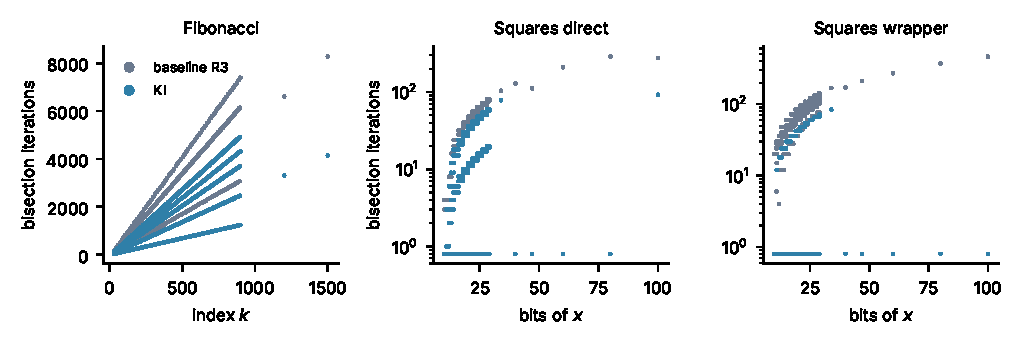
\includegraphics[width=0.98\textwidth]{../figures/fig2_cost.pdf}
\caption{Bisection iterations per input, baseline R3 versus KI. Squares panels on a log scale against the bit length of $x$; inputs with no bisection are drawn at $0.8$.}\label{fig:cost}
\end{figure}

\section{Updated knowledge ledger}\label{sec:ledger}
\begin{table}[h]\centering\small
\caption{Ledger after KI. Rows follow the five-source schema; the optimized selectors differ from R3 only in the third and fourth rows.}
\begin{tabular}{@{}p{0.27\textwidth}p{0.20\textwidth}p{0.22\textwidth}p{0.22\textwidth}@{}}\toprule
 & Fibonacci & Squares direct & Squares wrapper\\\midrule
Membership (controller) & $\isqrt$ test, $5x^2\pm4$ & $\isqrt$ test, $x=n^2$ & $\isqrt$ test, $x=n^2$\\
Fixed-modulus dispatch & $(x,y)\bmod 24$ & $n \bmod 24$ & $n \bmod 24$\\
State-only formulas, exact & \FibClosed/\FibTotal & \SqDClosed/\SqDTotal & \SqWClosed/\SqWTotal\\
Steps still needing recovery & \FibRec & \SqDRec & \SqWRec\\
Mean recoveries per route & \FibMeanRecB$\to$\FibMeanRecK & \SqDMeanRecB$\to$\SqDMeanRecK & \SqWMeanRecB$\to$\SqWMeanRecK\\
Certified formulas stored & \FibClosed & \SqDClosed & \SqWClosed\\
Route tables, edges & unchanged & unchanged & unchanged\\
Control states & \CtrlFib & \CtrlSqD & \CtrlSqW\\
External information & none & none & none\\\bottomrule
\end{tabular}
\end{table}
The reversible arithmetic still supplies legality (divisibility) and the bounded geometry of routes. The controller supplies membership, dispatch, route tables and, for the steps in the fourth row, parameter recovery. Under R3$'$ the three selectors compute their next term from the ready state, as R3 recorded; none of this addendum changes that, so the distinction knowing the target $\ne$ finding an admissible route $\ne$ generating the target intrinsically remains open at its third member.

\section{Gates}
\begin{center}\small
\begin{tabular}{@{}p{0.27\textwidth}p{0.08\textwidth}p{0.55\textwidth}@{}}\toprule
gate & status & evidence\\\midrule
Mathematical certification & pass & \StepsAll{} identities re-derived and equal to the stored table; all \ClosedAll{} formulas certified including branch sign; \NonClosed{} exact degrees with existence and lower-bound certificates\\
Domain certification & pass & identical outputs on all inputs of Section~\ref{sec:ki3}; every transition legal; refusals identical\\
Knowledge accounting & pass & ledger complete in the five-source schema; ``proved'' and ``not found'' kept separate (Section~\ref{sec:ki2})\\
Reproducibility & pass & deterministic verifier, hashes of sources, inputs and the frozen baseline (README)\\\bottomrule
\end{tabular}
\end{center}
\paragraph{Unverified assumptions.} (1)~SymPy exactness and Sturm counts; no proof assistant. (2)~Rank statements modulo a prime rely on Python integer arithmetic. (3)~The Galois step in Proposition~\ref{prop:tower} uses a cited standard theorem. (4)~The tower question for the \FieldPowTwo{} steps with $d\in\{4,8\}$ was not analysed. (5)~The frozen U2-001 evaluator uses floating-point lambdified labels at non-shortcut wrapper steps; agreement was observed up to $n=10^{15}$ and not proved beyond. (6)~Test ranges are finite; the identities, not the tests, carry the claim for all class members with $b\ge40$ resp.\ $t\ge t_0$. (7)~Cost counters are Python operation counts, not machine time. (8)~No literature priority search was made. (9)~Whether R3$'$ is the intended reading of Definition~2.1 remains a programme decision.

\section{Consequences}
The comparison between selectors is now an exact one: reversible arithmetic plus a few square roots determines most labels of the square selectors, but only about two fifths of the Fibonacci labels, and for $\NonClosed$ steps no formula with at most one root exists. The next experiments suggested by this are the proof-level lift of the tower analysis to the $d\in\{4,8\}$ steps, optimization of class~11 (which changes graph cost only), and a target-independent selector experiment, which has \emph{not} been run here. For primes, R3 stated only that no admissible selector has yet been constructed; that remains the position.

\begin{thebibliography}{9}\small
\bibitem{kosh} T.~Koshy, \emph{Fibonacci and Lucas Numbers with Applications}, Wiley.
\bibitem{sympy} A.~Meurer et al., SymPy: symbolic computing in Python, \emph{PeerJ CS} 3 (2017) e103.
\bibitem{lang} S.~Lang, \emph{Algebra}, Springer: Lüroth's theorem; Dedekind's factorization theorem and Galois groups of specializations.
\bibitem{sturm} Sturm's theorem for real root counting, e.g.\ in B.~Mishra, \emph{Algorithmic Algebra}, Springer.
\bibitem{r3} UNNS-U2-FP-R3 v001 and the frozen packages U1-BND, U2-001, U2-SQ, U2-FP, U2-FP-SYM (hashes in the README).
\end{thebibliography}

\appendix
\section{Step patterns}
\begin{description}[leftmargin=1.2em,itemsep=2pt,font=\normalfont\small]
\item[Fibonacci, $k \bmod 12$:] 0:\texttt{caRRRRqc} 1:\texttt{aRRRRRRRRq} 2:\texttt{aRRRRRRq} 3:\texttt{aRRRRqaq} 4:\texttt{caRRq} 5:\texttt{aRRRRRRRRq} 6:\texttt{aRRRRRRq} 7:\texttt{aRRqcaq} 8:\texttt{aRRRRq} 9:\texttt{aRRRRRRRRq} 10:\texttt{ccaRRcq} 11:\texttt{aRRRRRRqcRqc}
\item[Squares direct, $n \bmod 24$:] 0:\texttt{qRcRR} 1:\texttt{aqqR} 2:\texttt{qaqa} 3:\texttt{ccqa} 4:\texttt{cqRRR} 5:\texttt{aqqR} 6:\texttt{qaqa} 7:\texttt{ccqac} 8:\texttt{ccqac} 9:\texttt{aqqR} 10:\texttt{qaqa} 11:\texttt{ccqac} 12:\texttt{qRcRR} 13:\texttt{aqqR} 14:\texttt{qaqa} 15:\texttt{ccqa} 16:\texttt{cqRRR} 17:\texttt{aqqR} 18:\texttt{qaqa} 19:\texttt{ccqac} 20:\texttt{qaqa} 21:\texttt{aqqR} 22:\texttt{qaqa} 23:\texttt{ccqac}
\item[Squares wrapper, U2-001 class:] A:\texttt{qaqaqa} B:\texttt{qcccaqa} C:\texttt{qcaccqa} D:\texttt{qcccaqa} E:\texttt{qcaccqa} F:\texttt{qaqaqa} G:\texttt{qaqRRRqa} H:\texttt{qacqaqca} I:\texttt{qcacqaqa}
\end{description}

Letters: \texttt{c} constant, \texttt{a} affine in the state, \texttt{q} one $\isqrt$ of the state, \texttt{R} recovery.
\end{document}
